% !TEX encoding = ISO-8859-1
\chapter{Figuras das Bases Artificiais}
\label{ch:appendixa}

\section{Figuras com 10\% da classe minorit�ria}
\begin{figure}[H]
\center
	\mbox{%
		\subfigure[N�vel I de sobreposi��o]{\label{fig:orig100}%
			\includegraphics[scale=0.30]{imagens/outputs/ORIG_10_0.eps}} 
		\subfigure[N�vel II de sobreposi��o]{\label{fig:orig101}%
			\includegraphics[scale=0.30]{imagens/outputs/ORIG_10_1.eps}}
	}
	\mbox{%
		\subfigure[N�vel III de sobreposi��o]{\label{fig:orig105}%
			\includegraphics[scale=0.30]{imagens/outputs/ORIG_10_5.eps}}
		\subfigure[N�vel IV de sobreposi��o]{\label{fig:orig1010}%
			\includegraphics[scale=0.30]{imagens/outputs/ORIG_10_10.eps}}
    }
	\mbox{%
		\subfigure[N�vel V de sobreposi��o]{\label{fig:orig1015}%
			\includegraphics[scale=0.30]{imagens/outputs/ORIG_10_15.eps}} 
    }
  \caption{Bases artificiais com 10\% da classe minorit�ria}
  \label{fig:orig10}
\end{figure}

\section{Figuras com 5\% da classe minorit�ria}
\begin{figure}[H]
\center
	\mbox{%
		\subfigure[N�vel I de sobreposi��o]{\label{fig:orig50}%
			\includegraphics[scale=0.30]{imagens/outputs/ORIG_5_0.eps}} 
		\subfigure[N�vel II de sobreposi��o]{\label{fig:orig51}%
			\includegraphics[scale=0.30]{imagens/outputs/ORIG_5_1.eps}}
	}
	\mbox{%
		\subfigure[N�vel III de sobreposi��o]{\label{fig:orig55}%
			\includegraphics[scale=0.30]{imagens/outputs/ORIG_5_5.eps}}
		\subfigure[N�vel IV de sobreposi��o]{\label{fig:orig510}%
			\includegraphics[scale=0.30]{imagens/outputs/ORIG_5_10.eps}}
    }
	\mbox{%
		\subfigure[N�vel V de sobreposi��o]{\label{fig:orig515}%
			\includegraphics[scale=0.30]{imagens/outputs/ORIG_5_15.eps}} 
    }
  \caption{Bases artificiais com 5\% da classe minorit�ria}
  \label{fig:orig5}
\end{figure}




